
\chapter{序論}\label{chapter:序論}
第\ref{chapter:序論}章では,本研究の背景と先行研究,そして研究の目的を述べる.


\section{背景}

% 流れ
% 多脚ロボットの特徴と,不整地の移動に適していることを述べる
% 不整地の移動において,6脚であることによる利点を述べる
% 適応歩容の必要性を述べる
% 適応歩容の実現方法を述べる,そして,グラフ探索による手法を述べる

% 1.1.1 章
\subsection{不整地における多脚ロボットの活用}
レストランの配膳や倉庫の整理,発電所や工事現場の点検などさまざまな現場で
人間に代わって作業を行う移動ロボットの導入が検討されている\cite{cita:news_robot}.
導入されるロボットの移動様式は主にタイヤ,クローラを用いた移動や,脚を用いた移動がある.
タイヤやクローラを用いた移動は制御が容易で,高速で移動することができるため多くのロボットで用いられており,
実際に配膳や倉庫の整理などの作業を行う移動ロボットの導入が進められている\cite{Sotnik_Prospects_for_Introduction}.
身近な例としてはPudu社が開発したロボットのBellaBot\cite{Pudu_BellaBot}があげられるだろう.
しかし,タイヤを用いた移動では,急な段差を乗り越えることや,穴の開いた道を通ることができないため,不整地での移動には適していない.
クローラを用いた移動はタイヤに比べ不整地を踏破する能力に長けるが,
地面に与える影響が大きく環境にダメージを与えてしまう問題点がある.

脚を使用して移動を行うロボット(以下脚ロボット)はそのような不整地において活用するのに適した特徴をもつ.
文献\cite{Locomotion_for_difficult_terrain}では脚ロボットは他の移動様式を用いて移動するロボットに比べて,
以下に示すような利点があると述べられている.

\begin{itemize}
  \item 障害物をまたいで移動できるため,対地適応性が高い
  \item 脚接地点を離散的に選択できるため,環境に与える影響が小さい
  \item スリップすることなく全方向に移動できる
\end{itemize}

障害物をまたいで移動できることにより,
脚ロボットはタイヤでは移動できないような凹凸が激しい地形や,
不連続な地形においても移動することが可能である.
また,砂利で舗装された道のような,
クローラではスリップしてしまうような環境においても移動することが可能である.
この特徴を生かして,
実際に\figref{fig:nedo_spot}のようにBoston Dynamics Inc. によって開発された
4足歩行ロボットのSpot\cite{Boston_Dynamics_Spot}を用いて,
林業を行う山間地で作業を行う実証実験が行われている\cite{NEDO}.
山間地は斜面である上に,伐根作業によって木の根が残っているため凹凸が激しく,
タイヤやクローラでは移動が困難である.
しかし,脚ロボットであるSpotは障害物をまたいで移動することができるため,
このような環境での作業に適しており,
導入による人手不足の解消や,作業効率の向上が期待されている.

また,離散的に脚接地地点を選択できるため,
タイヤやクローラによる移動と比較して環境に与える影響が小さい.
この特徴を生かしたロボットの実例として,
韓国海洋科学技術院によって開発された6脚ロボットのCrabster\cite{J_Kim_Dexterous_Crabster}があげられる.
\figref{fig:crabster}に示したCrabsterは,流れの早い海底での作業を想定して開発されており,
6本の脚による移動を行うことや,4本の脚を海底に接地させ,
残りの2本の脚を用いて作業を行うことが可能である.
脚を用いた移動では海底の砂を大量に巻き上げることがないため\cite{J_Kim_Little_Crabster},
カメラを用いた観察や,センサを用いた地形の計測に優れている.
以上より,脚ロボットは対地適応性が高く,環境に与える影響が小さいため,
不整地での移動に適しているといえる.

\begin{figure}[htbp]
  \begin{center}
    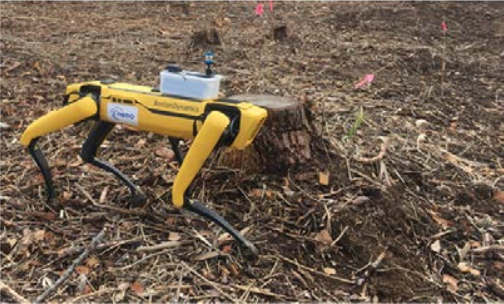
\includegraphics[width=90mm, clip]{figure/chapter1/NEDO.png}
    \caption{Demonstration Experiment with Spot}
    \label{fig:nedo_spot} % chktex 24
  \end{center}
\end{figure}

\begin{figure}[htbp]
  \begin{center}
    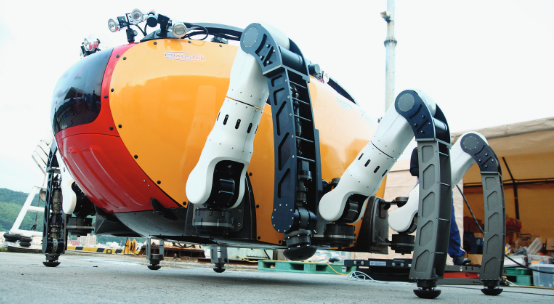
\includegraphics[width=90mm, clip]{figure/chapter1/crabster.png}
    \caption{Crabster}
    \label{fig:crabster} % chktex 24
  \end{center}
\end{figure}

このような特徴をもつ脚ロボットであるが,実際に不整地で活用された事例は多くない.
原因として,\cite{Locomotion_for_difficult_terrain}では
以下に示すような問題を脚ロボットが抱えているためと述べられている.

\begin{itemize}
  \item 脚の機構はアクチュエータの数が多いため,重量が大きくなってしまう
  \item 移動には歩行のための制御が必要であり,タイヤやクローラに比べて制御が複雑になる
\end{itemize}

多脚ロボットの積極的な活用を考えると,脚の機構の軽量化と,
歩行のための制御の手法が必要である.
そこで本研究では多脚ロボットの制御に着目し,
不整地における多脚ロボットの活用のための歩行の制御手法を論じることとする.

不整地で脚ロボットを歩行させることを前提に,脚ロボットの歩行形態について考える.
脚ロボットの歩行形態は大別して,動歩行と静歩行に分けられる.
静歩行とは,支持脚多角形とも呼ばれる,
地面に接地している脚をすべて結んでできる多角形上に重心をおき,
常に静的な安定性を保ちながら歩行することと定義される\cite{Hirose_Static_stability_criterion}.
それに対して動歩行とは静的には不安定であるが,動的に安定を保ちながら歩行することである.
静歩行では常に支持脚多角形上に重心を置くため,動歩行と比較して歩行速度が遅くなる.
しかし,動歩行は重心の位置や歩行の速度を踏まえた動的な制御が必要となるため,静歩行に比べて制御が複雑になる.
加えて不整地の歩行では地形の状態を考慮する必要があるため,より制御の難易度は高くなる.
そのため,静歩行を用いたほうが不整地歩行を実現しやすいことがわかる.

静歩行による不整地の歩行は,主に4脚以上の脚ロボットで研究されている.
なぜならば,2脚を有する脚ロボットは静的な安定性を保ちながら歩行する場合,
重心の位置が支持脚面積の中になるように制御する必要があるため,
実用的な歩行速度を得ることが難しいためである.
そのため,より早い静歩行には4脚以上の脚を有する脚ロボットが有利である.
本論文ではそのような4,6脚以上の脚を有する脚ロボットを多脚ロボットと呼ぶことにする.
制御を簡単にするため,多脚ロボットの脚数は少ないほうが望ましい.
実際に多くの研究において,静歩行が可能な最小の脚数を有する4脚ロボットや6脚ロボットが用いられている.
なかでも6脚ロボットは,1脚が故障しても静歩行を継続することが可能であるため耐故障性に優れている.
また,6脚ロボットは1度に最大3本の同時に遊脚することができるため,
4脚ロボットと比べ静歩行時の歩行速度が速くなる.
6脚ロボットは静歩行において,いくつかの4脚ロボットよりも優れた性能を持つが,
これらの特徴を生かすには4脚ロボットの制御に比べ,高度な制御が必要となる.

% 1.1.2 章
\subsection{固定歩容と自由歩容}
多脚ロボットが歩行を行う際には,脚を適切な順番で動かす必要がある.
脚ロボットの歩行中の脚を動かす順序や,脚を動かすタイミングのことを歩容と呼ぶ.
歩容にはさまざまな種類があるが,大別すると周期的に同じパターンの脚の動作を繰り返す固定歩容と,非周期的に脚を動かす自由歩容に分けられる.

固定歩容は自然界においても多く見られる歩容であり,動物の歩行や,昆虫の歩行などがこれにあたる.
代表的なものとしては,低速で4足歩行をする動物にみられるクロール歩容がある.
これは,歩行中に常に3本の脚が地面に接地しており,1本の脚が遊脚する歩容パターンである.
3本の脚が地面に接地しているため,常に静的な安定性を保つことができるが,1本づつしか脚を動かせないため,一般に歩行速度は遅い.

6足歩行する昆虫の中には,トライポッド歩容と呼ばれる歩容をとるものがある.
この歩容パターンでは,まず片側の前脚と後ろ脚,反対側の中央の脚を地面に接地させ,残りの3本の脚を遊脚させる.
次に,反対側の前脚と後ろ脚,片側の中央の脚を地面に接地させ,残りの3本の脚を遊脚させる動作を繰り返す.
この歩容では同時に3本の脚を地面に接地させることができるため,クロール歩容よりも歩行速度が速くなる.

固定歩容は平地において比較的高速かつ安定した歩行を実現することができるが,
不整地においては遊脚の可動範囲内の接地点が存在しない場合,歩容を維持することができない.
文献\cite{cita:satou_tripod_gait}では地形の変化を考慮して,
重心高さを変更させたり,胴体を傾けたりすることで常にトライポッド歩容をとれるように制御する手法が提案されているが,
6脚ロボットの持つ耐故障性を生かすためには,地形に応じた自由歩容パターンを生成する必要があるといえる.

% 1.1.3 章
\subsection{グラフ探索による自由歩容パターン生成手法}
自由歩容パターンを生成する手法として,グラフ探索による自由歩容パターン生成手法がある\cite{Prabir_Graph_search}.
これは,脚位置や動作を離散化することでロボットの歩容をグラフに落としこみ,
そのグラフを探索することによって数動作先までの歩容パターンの組み合わせを網羅的に調べ,最適な歩容パターンを選択する手法である.
この手法の特徴として,数動作先までを考慮して歩容パターンを生成するため,デッドロックに陥りにくいという点や,
効率的な歩容パターンを生成することができるという点が挙げられる.

しかし,グラフ探索による自由歩容パターン生成手法は,脚の本数が増えることで脚の動かし方の組み合わせが増えるため,
グラフの規模が大きくなり,実時間内の計算が困難になるという問題がある.
4脚ロボットにおいて,静的安定性を保ちながら歩行する場合,1度に遊脚することができる脚は1本であるため,
実時間内の計算は容易である.
だが,6脚ロボットは静的安定性を保ちながら最大3本の脚を遊脚することができるため,
グラフの規模が大きくなり,実時間内の計算が困難になる.
この問題を解決するためにPrabirらは歩容をウェーブ歩容に限定することで,
グラフの規模を小さくすることに成功した\cite{Prabir_Graph_search_Six},
また新らは歩容をトライポッド歩容に限定することで\cite{Arata_Graph_search_Six},
同様にグラフの規模を小さくしている.
これらの手法は歩容を限定することでグラフの規模を小さくすることに成功しているが,
ロボットの行う動作の種類が限定されてしまうという問題がある.

そこで本研究室ではロボットの動作を制限することなく,グラフ探索による自由歩容パターン生成手法を6脚ロボットに適用するため,
離散化された脚位置の組み合わせを利用してグラフの階層構造化を行った.
また,自由歩容パターン生成による接地地点の計算と脚軌道の生成を分離した.
これらによって,グラフ探索による自由歩容パターン生成手法を6脚ロボットに適用することが可能になった.

本研究室では,ロボットを動作させる地形やロボットの動作によって段階的に開発を行っており,
これまでに2次元空間において,直進動作\cite{Oki_Graph_search},目的姿勢での停止\cite{Nakaoka_Graph_search},
旋回動作\cite{Shina_Graph_search}を行うための歩容パターン生成手法の実装に成功した.
また3次元空間においても,脚位置の離散化方法を3次元に適応させたことで\cite{Miura_Graph_search},
直進動作\cite{Hato_Graph_search}を行うための歩容パターン生成手法の実装に成功した.

\section{本研究の目的}
これまでの研究によって,3次元の不整地において,重心高さを変更しつつ,
自由歩容パターン生成を行うことが可能となった.
しかし低頻度ではあるが,グラフ探索に成功したとしても脚軌道が生成できず,その歩容パターン通りに歩行することできなくなり,
動作を停止してしまう問題が生じてしまった.

これは,グラフ探索と脚軌道生成を分離したことによって生じた問題であり,
先行研究では継続的にこの問題について言及されていたが,
グラフの規模を大幅に増大させることなく,また歩容生成の成功率を低下させることなく,
この問題を解決することはできなかった.

そこで本論文では,常に脚軌道生成に成功するような歩容パターン生成手法を提案し,
脚軌道生成の失敗による動作停止を防ぐことを目的とする.

\section{本論文の構成}
本論文は,全6章から構成される.

第2章「歩容パターンの再評価手法の提案」では,常に脚軌道生成が可能になる手法として,
歩容パターンの再評価手法を提案し,その機能を述べる.

第3章「歩容パターンの再評価手法の実装」では,提案したプログラムの実装方法を述べる.

第4章「再評価手法の有効性の確認のための歩行シミュレーション」では,
提案手法を用いたシミュレーション実験の結果を述べる.

第5章「常に脚軌道生成が可能な自由歩容パターン生成手法を用いた実機による歩行実験」
では,提案手法を用いた実機試験の結果を述べる.

第6章「結論」では本論文の結論と今後の課題を述べる.
